
\section{Evaluation}
This section demonstrates how we model and synthesize collectives for
two multi-GPU systems with proprietary interconnects used for training
large deep learning models. In both cases, we demonstrate 1) how to
model the interconnect using \tool, 2) what transport we utilize in
lowering synthesized collectives, and 3) the Pareto-frontier of
algorithms we find for the respective interconnects.

\subsection{Hardware}
The following section describes the hardware topology we model for our
NVIDIA and AMD machines.

\subsubsection{NVIDIA DGX-1: 8 V100 GPUs}
A DGX-1 is a multi-GPU server sold directly by NVIDIA in addition to
being a pay-as-you-go rental option in most cloud providers.  It
contains two 20-core Intel Xeon E5-2698 v4 processors with 512 GB DRAM
split across the two sockets, along with 8 NVIDIA V100 GPUs, each with
32 GB of HBM2 memory. The GPUs are connected using NVIDIA's
proprietary NVLink interconnect; each GPU has 6 25 GB/s NVLink ports.
Figure~\ref{fig:dgx1-topo} shows the topology: the 8 GPUs are
interconnected with 2 non-overlapping Hamiltonian cycles.  One of
those cycles has two NVLink connections between each pair of GPUs. The
GPUs are also connected to the CPUs by PCIe 3.0 x16 links, but we do
not use them due to the wide disparity between per-GPU NVLink and PCIe
bandwidth ($\sim$150~GB/s vs. $\sim$14~GB/s). We also run synthesis on
this platform.

\subsubsection{Gigabyte Z52: 8 AMD MI50 GPUs}
A Gigabyte Z52 system is a consumer grade multi-GPU system. It has two
64-core AMD EPYC 7002 processors with 1 TB DRAM split across the two
sockets, as well as 8 AMD MI50 GPUs, each with 32 GB of HBM2 memory. 4
GPUs are connected to each socket with PCIe links, denoted by a box in
Figure~\ref{fig:amd-topo}. Like NVIDIA, AMD also provides a
proprietary high-speed interconnect called xGMI that links GPUs
together.  Each blue line is an xGMI link between a pair of GPUs. Note
that the xGMI connections build two disconnected islands: 3 GPUs per
island are on 1 socket while a lone GPU is on the \emph{other} socket
(i.e., GPU 1 and 5). The Gigabyte system uses PCIe 4.0 x16 links with
measured bandwidth ($\sim$27 GB/s) that approaches xGMI's measured
bandwidth ($\sim$33 GB/s). As such, we use PCIe to connect the rings.

\begin{figure}[tbp]
  \centering
  \includegraphics[page=2,width=0.8\columnwidth]{figures/topos}
  \caption{Topology of a Gigabyte MI50 8 GPU AMD system.}
  \label{fig:amd-topo}
  \end{figure}

\subsection{Modeling Bandwidth Constraints}
The hardware in this chapter has distinct and interesting topologies.
This section describes how we model those respective topologies in
\tool.

\subsubsection{NVIDIA DGX-1: 8 V100 GPUs}
Each NVLink connection is point-to-point; thus our bandwidth
constraints are simply the enumeration of each pair of GPUs connected
via NVLink. As each NVLink connection can send 1 chunk per round,
$\bw$ has entries $(\{(n,n')\},1)$ for each pair of GPUs in one cycle
and entries $(\{(n,n')\},2)$ for GPUs in the other.

\subsubsection{Gigabyte Z52: 8 AMD MI50 GPUs}
Unlike NVLink, xGMI connections are not simply point-to-point but also
transparently act as a router.  For example, GPU 2 can send a message
to GPU 3 even though they lack a physical connection: GPU 0 routes
messages on GPU 2's behalf.  However, this utilizes multiple links,
and thus if GPU 0 concurrently sends a message to GPU 3, it can expect
half the bandwidth of the link.  We thus only model the direct
connections in Figure~\ref{fig:amd-topo}.  One way to connect the
rings is to utilize PCIe and let GPU 1 connect to all other GPUs
within its same socket (0, 2, and 3) and GPU 5 connect to GPUs within
its same socket (4, 6, and 7).  Because PCIe is shared, we could also
enforce that only 1 PCIe connection occurs on every round, per socket.
%
% remove if need space
For example, the entry in $\bw$ for the left socket is
$(\{(0,1),(1,0),(1,2),(2,1),(1,3),(3,1)\},1)$.
%
However, we were unable to utilize both xGMI and PCIe at the same time
so our model of the bandwidth ignores the dotted xGMI connections in
Figure~\ref{fig:amd-topo}.  As such, we explicitly model the topology
as a ring with GPUs 1 and 5 connecting the xGMI islands. Lastly,
because the bisection bandwidth between the two xGMI islands is
limited by the PCIe links that connect them, any bandwidth optimal
algorithm will be limited by the bandwidth of these PCIe links.
Therefore, we model the same $\beta$ cost for xGMI and PCIe and assume
all links can send a single chunk per step.
%Finally, we noticed a single kernel was not able to utilize both xGMI
%and PCIe at the same time so we restrict each GPU to using only two
%of the potentially three possible links.


\subsection{NCCL and RCCL Baselines}
We use NCCL (version 2.7.8-1) and RCCL (installed from ROCm 3.5.0) for
baselines on NVIDIA and AMD hardware, respectively.  NCCL is a
hand-written and optimized communication library from NVIDIA. RCCL is
a port of NCCL that uses the ROCm HIP compiler and targets AMD
hardware. They share the same core algorithms and differ only in how
they interact with the underlying hardware.

\newcolumntype{H}{>{\setbox0=\hbox\bgroup}c<{\egroup}@{}}

\begin{table}[bp]
\caption{NCCL hand-written collectives and their chunks and steps. }
\begin{tabularx}{\columnwidth}{@{}Xlll@{}}
\toprule
Collective &$\chunk$ & $\steps$ & $\rounds$ \\
\midrule
\allgather/\reducescatter & 6 & 7 & 7 \\
\allreduce & 48 & 14 & 14 \\
\broadcast/\reduce  & $6m$ & $6+m$ & $6+m$ \\
\bottomrule
\end{tabularx}

\label{table:nccl}
\end{table}

Table~\ref{table:nccl} gives an overview of the collectives that NCCL
implements and number of chunks and steps they use on a \dgxone.
NCCL's algorithms are all based on either rings or trees. However,
Table~\ref{table:nccl} uses only ring algorithms, as we observed that
on DGX-1 NCCL's trees are just simple paths, which are no better than
using rings for any input size.
% As of NCCL version 2.8.7-1, the tree based algorithm is only used in
% \allreduce and upon manual inspection, the tree on our \dgxone node
% is actually a ring.

Our analysis of the chunks ($\chunk$), steps ($\steps$), and
rounds($\rounds$) is from our manual inspection of the NCCL source.
For \reduce and \broadcast NCCL implements a pipelined algorithm,
which chooses a multiplier $m$ such that chunks stay approximately
equally sized. Their running times are then $(6+m) \cdot \alpha +
\frac{6+m}{6m}\cdot L \cdot \beta$ and they get closer to bandwidth
optimality as $m$ gets larger.

As we show in the next section, \tool{} is able to synthesize all
these NCCL collectives and more, including \scatter, \gathercoll, and
\alltoall.
%Further, for each collective, \tool{} synthesizes many more
%Pareto-optimal algorithms.

% synhtesis looks fast but it is solving a hard problem and our
% results are due to efforts noted above.  Naive encoding does not
% scale... maybe remove some symmetry?

\subsection{Synthesizing Collective Algorithms}
Table~\ref{fig:dgxone:syn} and Table~\ref{fig:amd:syn} enumerate
various algorithms we synthesize for NVIDIA \dgxone and Gigabyte's
\amd architecture.  For each collective, we synthesize a latency and
bandwidth optimal implementation, along with others that exist at
various points along the latency-bandwidth curve. The first column
combines collectives which are the inverse of each other (i.e.,
\scatter and \gathercoll) and those that can be reduced to the
\broadcasting collective using the reduction explained in
Section~\ref{sec:reduction} (e.g. \reduce to \broadcast).

\subsubsection{Optimality}
Note we find many latency and bandwidth optimal algorithms for each
collective, as we search over $k$-synchronous algorithms for different
values of $k$. Consider the \allgather collective: we find many
algorithms with various numbers of steps. However, the latency optimal
algorithms (2 steps) dominate all others in the $\alpha$ term of the
cost model.  Likewise, the bandwidth optimal algorithms dominate all
others with their low ratio of rounds to chunks ($7/6$). We
synthesized algorithms in the $0$-synchronous class ($\rounds =
\chunk$) as the code generation is much easier.

%There are various reasons to synthesize more than the lowest latency
%bandwidth-optimal and highest bandwidth latency-optimal algorithms:
%for example, any algorithm with $R == S$ is straightforward to
%implement as each step has a logical barrier between them.

Note that NCCL's \allgather algorithm is bandwidth optimal, and while
it is also the lowest latency algorithm that NCCL provides, it is not
latency optimal. We are able to synthesize both a bandwidth optimal
algorithm with better latency (6-chunks 3-steps 7-rounds), as well as
a latency optimal algorithm. In general, our synthesized latency
optimal algorithms have no counterpart in NCCL and our bandwidth
optimal algorithms are better than NCCL's for \allgather, \broadcast,
and \reduce.

%See Section~\ref{sec:pareto:optimal} for a discussion of how latency
%and bandwidth optimality relate to Pareto-optimality.

\begin{table}[tbp]
\caption{\dgxone collectives with chunks ($\chunk$), steps ($\steps$) and rounds ($\rounds$).  }
\begin{tabularx}{\columnwidth}{@{}lHlllXHr@{}}
\toprule
Collective & Topology & $\chunk$ & $\steps$ & $\rounds$ & Optimality &
Running Time & Time \\
\midrule
\allgather & \dgxone & 1 & 2 & 2 &Latency&$2 \cdot \alpha + 2\cdot L
\cdot \beta$& 0.3 s\\
(\reducescatter)& \dgxone & 2 & 3 & 3 &&$3 \cdot \alpha + 3/2\cdot L
\cdot \beta$& 0.8 s\\
 & \dgxone & 3 & 4 & 4 &&$4 \cdot \alpha + 4/3\cdot L \cdot \beta$&
 1.5 s\\
 & \dgxone & 4 & 5 & 5 &&$5 \cdot \alpha + 5/4\cdot L \cdot \beta$&
 2.3 s\\
 & \dgxone & 5 & 6 & 6 &&$6 \cdot \alpha + 6/5\cdot L \cdot \beta$&
 3.3 s\\
 & \dgxone & 6 & 7 & 7 &Bandwidth&$7 \cdot \alpha + 7/6\cdot L \cdot
 \beta$& 4.6 s\\
 & \dgxone & 6 & 3 & 7 &Bandwidth&$3 \cdot \alpha + 7/6\cdot L \cdot
 \beta$& 6.6 s\\
 & \dgxone & 2 & 2 & 3 &Latency&$2 \cdot \alpha + 3/2\cdot L \cdot
 \beta$& 0.9 s\\
\hline
\allreduce & \dgxone & 8  &4  &4&Latency&$4 \cdot \alpha + 1/2\cdot L
\cdot \beta$& 0.3 s\\
  & \dgxone & 16 &6  &6&&$6 \cdot \alpha + 3/8\cdot L \cdot \beta$&
  0.6 s\\
  & \dgxone & 24 &8  &8&&$8 \cdot \alpha + 1/3\cdot L \cdot \beta$&
  1.3 s\\
  & \dgxone & 32 &10 &10&&$10 \cdot \alpha + 5/16\cdot L \cdot \beta$&
  2.9 s\\
  & \dgxone & 40 &12 &12&&$12 \cdot \alpha + 3/10\cdot L \cdot \beta$&
  5.6 s\\
  & \dgxone & 48 &14 &14&Bandwidth&$14 \cdot \alpha + 7/24\cdot L
  \cdot \beta$& 12.8 s\\
  & \dgxone & 48 &6  & 14&Bandwidth&$6 \cdot \alpha + 7/24\cdot L
  \cdot \beta$& 23.0 s\\
  & \dgxone & 16 &4  &6&Latency&$4 \cdot \alpha + 3/8\cdot L \cdot
  \beta$& 0.8 s\\
\hline
\broadcast & \dgxone & 2 & 2 & 2 &Latency&$2 \cdot \alpha + 1\cdot L
\cdot \beta$& 0.1 s\\
(\reduce) & \dgxone & 6 & 3 & 3 &&$3 \cdot \alpha + 1/2\cdot L \cdot
\beta$& 0.3 s\\
 & \dgxone & 12 & 4 & 4 &&$4 \cdot \alpha + 1/3\cdot L \cdot \beta$&
 1.0 s\\
 & \dgxone & 18 & 5 & 5 &&$5 \cdot \alpha + 5/18\cdot L \cdot \beta$&
 8.5 s\\
 & \dgxone & 6 & 3 & 5 &&$3 \cdot \alpha + 5/6\cdot L \cdot \beta$&
 0.9 s\\
\hline
\gathercoll & \dgxone & 1 & 2 & 2 &Latency&$2 \cdot \alpha + 2\cdot L
\cdot \beta$& 0.3 s\\
(\scatter) & \dgxone & 2 & 3 & 3 &&$3 \cdot \alpha + 3/2\cdot L \cdot
\beta$& 0.9 s\\
  & \dgxone & 3 & 4 & 4 &&$4 \cdot \alpha + 4/3\cdot L \cdot \beta$&
  1.6 s\\
  & \dgxone & 4 & 5 & 5 &&$5 \cdot \alpha + 5/4\cdot L \cdot \beta$&
  2.7 s\\
  & \dgxone & 5 & 6 & 6 &&$6 \cdot \alpha + 6/5\cdot L \cdot \beta$&
  3.8 s\\
  & \dgxone & 6 & 7 & 7 &Bandwidth&$7 \cdot \alpha + 7/6\cdot L \cdot
  \beta$& 6.0 s\\
  & \dgxone & 6 & 3 & 7 &Bandwidth&$3 \cdot \alpha + 7/6\cdot L \cdot
  \beta$& 11.4 s\\
  & \dgxone & 2 & 2 & 3 &Latency&$2 \cdot \alpha + 3/2\cdot L \cdot
  \beta$& 1.0 s\\
\hline
\alltoall & \dgxone & 8 & 3 & 3 &&$3 \cdot \alpha + 3/8\cdot L \cdot
\beta$& 2.6 s\\
  & \dgxone & 8 & 2 & 3 &Latency&$2 \cdot \alpha + 3/8\cdot L \cdot
  \beta$& 3.0 s\\
  & \dgxone & 24 & 8 & 8 &Bandwidth&$8 \cdot \alpha + 1/3\cdot L \cdot
  \beta$& 133.7 s\\
  & \dgxone & 24 & 2 & 8 &Both&$2 \cdot \alpha + 1/3\cdot L \cdot
  \beta$& 24.3 s\\
\bottomrule
\end{tabularx}

%For \reducescatter and \scatter $\chunk$ should be multiplied by 8.
\label{fig:dgxone:syn}
\end{table}

\begin{table}[tbp]
  \caption{\amd collectives with chunks ($\chunk$), steps ($\steps$) and rounds ($\rounds$). }
  \begin{tabularx}{\columnwidth}{@{}lHlllXHr@{}}
\toprule
Collective & Topology & $\chunk$ & $\steps$ & $\rounds$ & Optimality &
Running Time & Time \\
\midrule
\allgather & \amd & 1 & 4 & 4 &Latency&$4 \cdot \alpha + 4\cdot L
\cdot \beta$& 0.5 s\\
(\reducescatter) & \amd & 2 & 7 & 7 &Bandwidth&$7 \cdot \alpha +
7/2\cdot L \cdot \beta$& 1.3 s\\
 & \amd & 2 & 4 & 7 &Both&$4 \cdot \alpha + 7/2\cdot L \cdot \beta$&
 1.7 s\\
\hline
\allreduce & \amd & 8 &8&8&Latency&$8 \cdot \alpha + 1\cdot L \cdot
\beta$& 0.4 s\\
 & \amd & 16 &14&14&Bandwidth&$14 \cdot \alpha + 7/8\cdot L \cdot
 \beta$& 0.9 s\\
 & \amd & 16 &8&14&Both&$8 \cdot \alpha + 7/8\cdot L \cdot \beta$& 1.6
 s\\
\hline
\broadcast & \amd & 2 & 4 & 4 &Latency&$4 \cdot \alpha + 2\cdot L
\cdot \beta$& 0.1 s\\
(\reduce) & \amd & 4 & 5 & 5 &&$5 \cdot \alpha + 5/4\cdot L \cdot
\beta$& 0.2 s\\
 & \amd & 6 & 6 & 6 &&$6 \cdot \alpha + 1\cdot L \cdot \beta$& 0.3 s\\
 & \amd & 8 & 7 & 7 &&$7 \cdot \alpha + 7/8\cdot L \cdot \beta$& 0.5
 s\\
 & \amd & 10 & 8 & 8 &&$8 \cdot \alpha + 4/5\cdot L \cdot \beta$& 0.6
 s\\
\hline
\gathercoll & \amd & 1 & 4 & 4 &Latency&$4 \cdot \alpha + 4\cdot L
\cdot \beta$& 0.4 s\\
(\scatter) & \amd & 2 & 4 & 7 &Both&$4 \cdot \alpha + 7/2\cdot L \cdot
\beta$& 1.8 s\\
\hline
\alltoall & \amd & 8 & 4 & 8 &Both&$4 \cdot \alpha + 1\cdot L \cdot
\beta$& 8.2 s\\
\bottomrule
\end{tabularx}
%For \reducescatter and \scatter $\chunk$ should be multiplied by 8.
\label{fig:amd:syn}
\end{table}


\subsubsection{Synthesizing all collectives}
Collective communication libraries need to support a large and diverse
set of hardware architectures.  Efficiently implementing latency and
bandwidth optimal algorithms for various topologies is time-consuming
and error-prone. \tool's synthesis based approach allows it to easily
extend the set of algorithms through search: \tool{} synthesizes
algorithms for \alltoall, \gathercoll and \scatter where no such
counterparts exist in NCCL.

\subsubsection{Synthesis time}
The longest synthesis time is just over 2 minutes and most of the time
under 10 seconds.  The synthesis problem is non-trivial and its
complexity is defined by both the collective, as well as the hardware
topology we synthesize for. The clever encoding described in
Section~\ref{sec:encoding} was critical for achieving these fast
synthesis times. As a point of comparison, synthesizing the 24-chunk
8-step bandwidth-optimal \alltoall algorithm with a more direct
encoding with a Boolean variable for each tuple $(c, n, n', s) \in
\sends$ did not finish within 60 minutes. With the better encoding the
synthesis finishes in just over 2 minutes.

\subsection{Performance Evaluation}
In this section, we compare \tool's generated algorithms with NCCL and
RCCL on the NVIDIA and AMD hardware.  Our code generation uses a
protocol similar to the simple protocol (i.e., NCCL\_PROTO=Simple).
Thus, we use NCCL with the simple protocol as our baseline. We
investigate the performance of \allgather, \allreduce, and \alltoall
as they are popular primitives in different workloads including
machine learning. For each hardware platform and collective, we
generate multiple algorithms; for each algorithm, we lower using (1) a
single kernel-launch, or (2) multiple \texttt{cudaMemcpy} calls with
one per step. Each algorithm uses a push model for copying and when
\tool{} is compared with NCCL, we exhaustively search the size and the
number of thread blocks and report the best performing combination for
both \tool{} and NCCL. See Section~\ref{sec:lowering} for more
details.


Figure~\ref{fig:dgx1-res-allgather} compares \tool's generated code
for \allgather with NCCL's \allgather. A point on
Figure~\ref{fig:dgx1-res-allgather-avglat} ($x$,$y$) shows the running
time in $y$ milliseconds as a function of send input buffer size in
$x$ Kbytes while a point on
Figure~\ref{fig:dgx1-res-allgather-speedup} shows the $y$ speedup of
\tool's generated code over NCCL's \allgather as a function of send
input buffer size in $x$ Kbytes. We plot one line per algorithm
denoted as $(\chunk, \steps, \rounds)$ for respectively chunks, steps,
and rounds as defined in Table~\ref{fig:dgxone:syn}. To show the
impact of our lowering, we plot two versions of a bandwidth optimal
algorithm $(6,7,7)$ (which utilizes a push-copy) and $(6,7,7)$
\texttt{cudaMemcpy}.  The latter of which shows the significant impact
lowering can have on the performance. To simplify the figure, we only
show algorithms that were faster on at least one input size we
experimented with. As it can be seen from the lines, \tool{} is up-to
$2.2\times$ faster than NCCL's \allgather on small sizes and
$1.14\times$ faster on larger sizes. It is possible for \tool{} to
automatically switch between multiple implementations based on the
input size. In which case, \tool{} will consistently outperform NCCL.

\begin{figure}[tbp]
  \centering
  \subfloat[Average latency\label{fig:dgx1-res-allgather-avglat}]{
    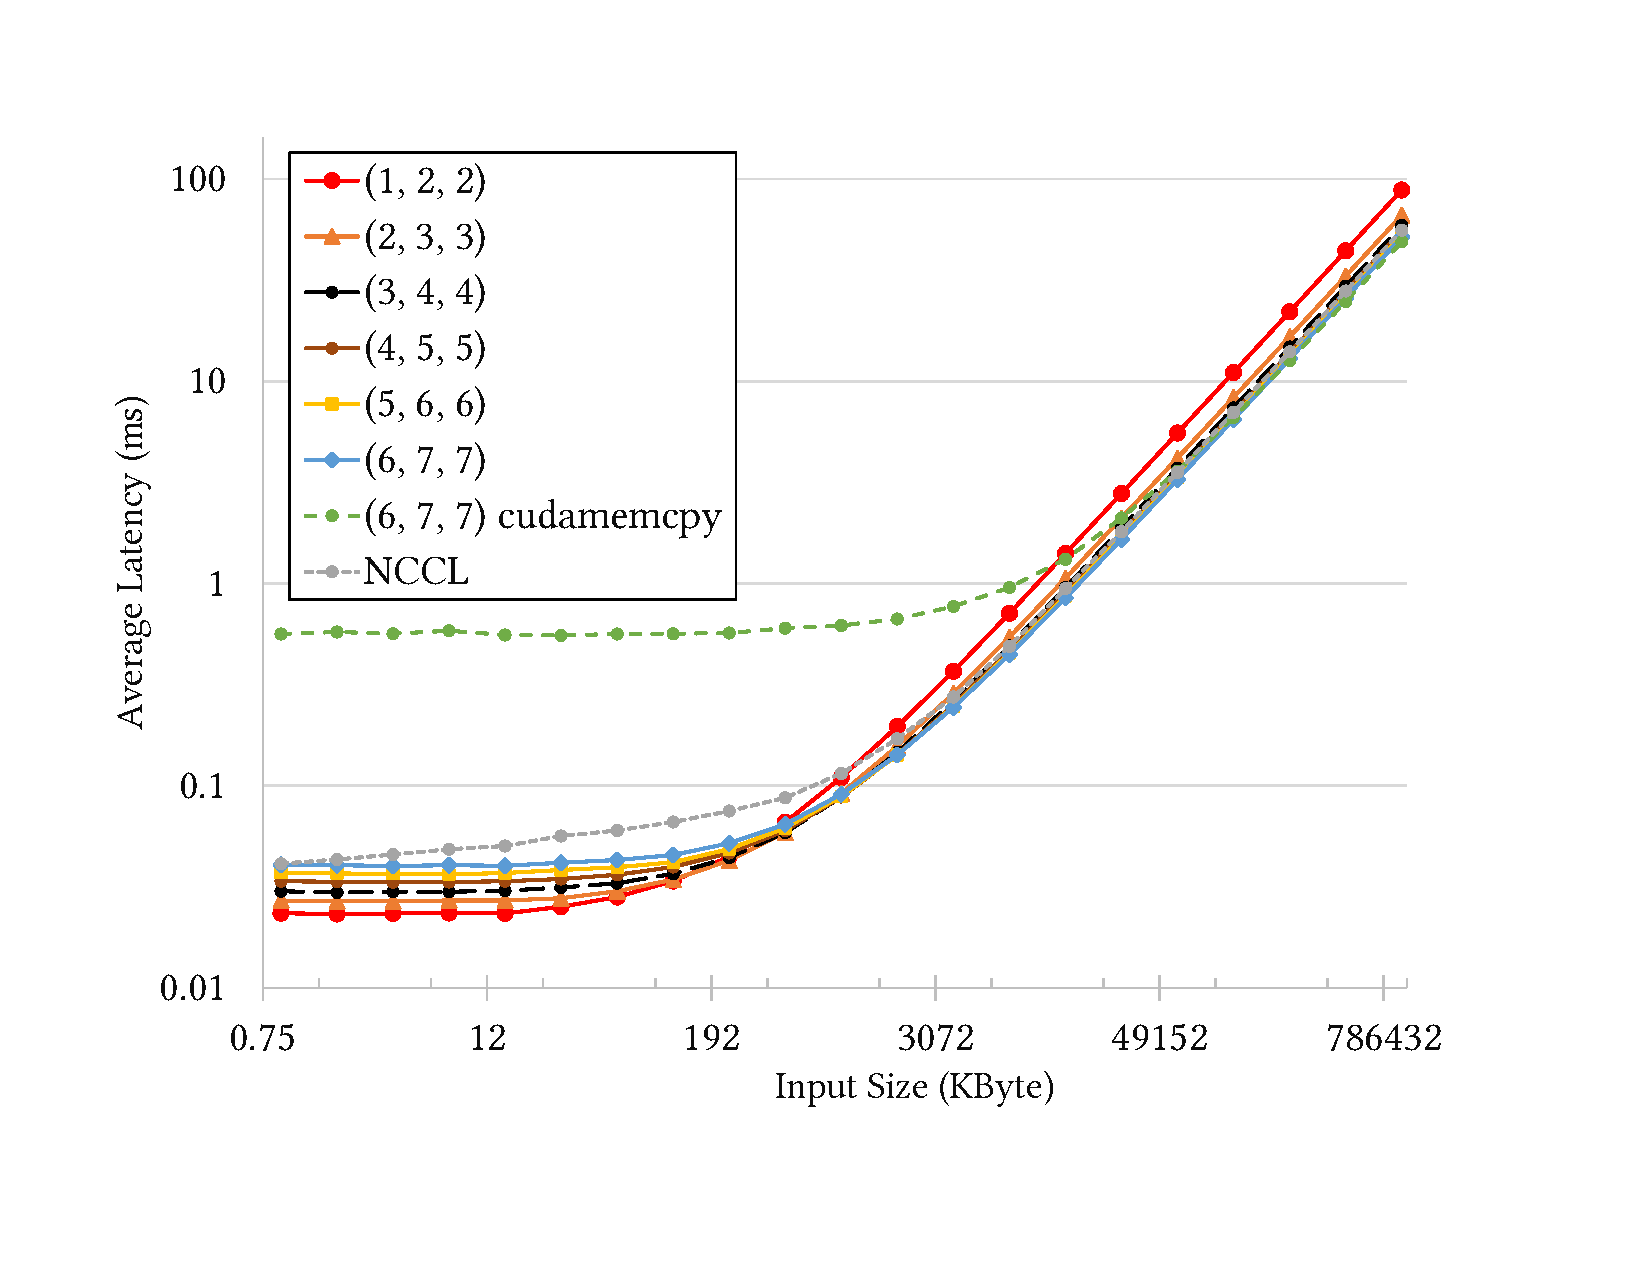
\includegraphics[page=1,width=0.84\columnwidth]{figures/evals-camera-ready}
  }
  \hfill
  \subfloat[Speedup\label{fig:dgx1-res-allgather-speedup}] {
    \includegraphics[page=2,width=0.84\columnwidth]{figures/evals-camera-ready}
  }
  \caption{\allgather performance comparison with NCCL.}
  \label{fig:dgx1-res-allgather}
\end{figure}

\begin{figure}[tbp]
  \centering
  \subfloat[Average latency\label{fig:dgx1-res-allreduce-avglat}] {
    \includegraphics[page=3,width=0.84\columnwidth]{figures/evals-camera-ready}
  }
  \hfill
  \subfloat[Speedup\label{fig:dgx1-res-allreduce-speedup}] {
    \includegraphics[page=4,width=0.84\columnwidth]{figures/evals-camera-ready}
  }
  \caption{\allreduce performance comparison with NCCL.}
  \label{fig:dgx1-res-allreduce}
\end{figure}


Likewise, Figure~\ref{fig:dgx1-res-allreduce} shows the running time
in milliseconds (Figure~\ref{fig:dgx1-res-allreduce-avglat}) or
speedup (Figure~\ref{fig:dgx1-res-allreduce-speedup}) for \allreduce
as a function of the receive input size.  Each line denotes $(\chunk,
\steps, \rounds)$ for respectively chunks, steps, and rounds,
respectively. With the exception of $4$ middle sizes, \tool{} beats
NCCL's \allreduce with an 8-chunk algorithm for small input sizes by
up-to $1.8\times$ and with a 48-chunk algorithm for large input sizes
by up-to $1.06\times$.

\alltoall is a complex algorithm which is very difficult to write
efficiently by hand. Unlike the prior collectives, NCCL does not
natively support \alltoall; instead, NCCL suggests using $N$
point-to-point exchanges (for $N$ GPUs) and thus its resulting
algorithm is neither bandwidth nor latency optimal.  Because \tool{}
uses program synthesis to generate optimal algorithms, it is able to
synthesize three \alltoall{} algorithms in a matter of minutes.
Figure~\ref{fig:dgx1-res-alltoall-avglat} shows the latency in
milliseconds of \tool{} and NCCL as a function of input size while
Figure~\ref{fig:dgx1-res-alltoall-speedup} shows speedup over NCCL
again as a function of input size.  Each line denotes $(\chunk,
\steps, \rounds)$ for respectively chunks, steps, and rounds and
demonstrates a speedup of over $6.8\times$ for large input sizes and
over $1.4\times$ for small input sizes, depending on whether we pick a
latency or bandwidth optimal implementation from \tool.  This
significant speedup really shows off the power of \tool's automated
approach to building algorithms tailored specifically to a hardware
architecture.

\begin{figure}[tbp]
  \centering
  \subfloat[Average latency\label{fig:dgx1-res-alltoall-avglat}]{
    \includegraphics[page=5,width=0.84\columnwidth]{figures/evals-camera-ready}
  }
  \hfill
  \subfloat[Speedup\label{fig:dgx1-res-alltoall-speedup}] {
    \includegraphics[page=6,width=0.84\columnwidth]{figures/evals-camera-ready}
  }
  \caption{\alltoall performance comparison with NCCL.}
  \label{fig:dgx1-res-alltoall}
\end{figure}

Lastly, we demonstrate \allgather on the Gigabyte AMD workstation.
Like the other plots, a point on Figure~\ref{fig:amd-res-allgather}
($x$,$y$) shows the latency or speedup $y$ for \allgather as a
function of the receive input size in bytes $x$.  We plot two
algorithms, $(1,4,4)$ and $(2,7,7)$; it is clear that (i) the lower
latency algorithm $(1,4,4)$ is better at smaller input sizes, (ii) the
higher bandwidth algorithm $(2,7,7)$ is faster for large input sizes,
and (iii) \tool's generated code is faster than RCCL for large sizes
but slower for medium and small sizes. The Gigabyte machine, in
particular, is new hardware and \tool{} can synthesize new algorithms
and implementations for it; this shows \tool{} can help design future
interconnects and co-design them with communication libraries.

These graphs in concert show that \tool{} is able to synthesize
algorithms along the Pareto-optimal frontier and also lower than to
hardware so as to be competitive with a hand optimized baseline.

\begin{figure}[tbp]
  \centering
  \subfloat[Average latency\label{fig:amd-res-allgather-avglat}]{
    \includegraphics[page=7,width=0.84\columnwidth]{figures/evals-camera-ready}
  }
  \hfill
  \subfloat[Speedup\label{fig:amd-res-allgather-speedup}] {
    \includegraphics[page=8,width=0.84\columnwidth]{figures/evals-camera-ready}
  }
  \caption{\allgather performance comparison with RCCL.}
  \label{fig:amd-res-allgather}
\end{figure}
